% Wave Grid 3x3: write-in worksheet for sighted students.
% Build the student copy:  latexmk -pdf write-in-worksheet.tex
% Build the answer key:    latexmk -pdf -jobname=write-in-worksheet-key \
%                            -usepretex='\def\withanswers{1}' write-in-worksheet.tex
% (build.sh does both.)
\documentclass[11pt,addpoints]{exam}
\ifdefined\withanswers\printanswers\fi
\usepackage[letterpaper,margin=0.7in]{geometry}
\usepackage[T1]{fontenc}
\usepackage{lmodern}
\usepackage{graphicx}
\usepackage{array}
\usepackage{tikz}
\usepackage{siunitx}
\usepackage[hidelinks]{hyperref}
\renewcommand{\solutiontitle}{\noindent\textbf{Answer:}\enspace}
\unframedsolutions
\SolutionEmphasis{\color{blue!60!black}}
\pagestyle{headandfoot}
\firstpageheader{}{}{}
\runningheader{Feeling a Wave}{}{Wave Grid 3\(\times\)3 worksheet\ifprintanswers\ (answer key)\fi}
\footer{\footnotesize CC BY 4.0 \textperiodcentered\ University of Scranton Amateur Radio Club (W3USR) \textperiodcentered\ github.com/w3usr/handiham-tactile-aids}{}{\footnotesize Page \thepage\ of \numpages}
\renewcommand{\questionlabel}{\textbf{\thequestion.}}
\pointsinrightmargin
\pointpoints{pt}{pts}

\newcommand{\blank}[1][3cm]{\underline{\hspace{#1}}}

\begin{document}

\begin{center}
{\LARGE\bfseries Feeling a Wave: Amplitude and Frequency}\\[4pt]
{\large Wave Grid 3\(\times\)3 worksheet\ifprintanswers\ \textendash\ answer key\fi}
\end{center}

\vspace{4pt}
\noindent Name \blank[6cm] \hfill Date \blank[3.5cm]

\vspace{10pt}
\noindent The \textbf{Wave Grid} is a 3D-printed board with nine tiles. Each tile carries a wave you can
feel with your fingertips. It was designed so that blind students can learn about waves by touch,
and it works just as well for everyone else. If you have the board, use it. If not, use the
drawings below: each box is the side view of one tile, drawn at \textbf{actual size} when this
page is printed at 100\%.

\vspace{6pt}
\begin{center}
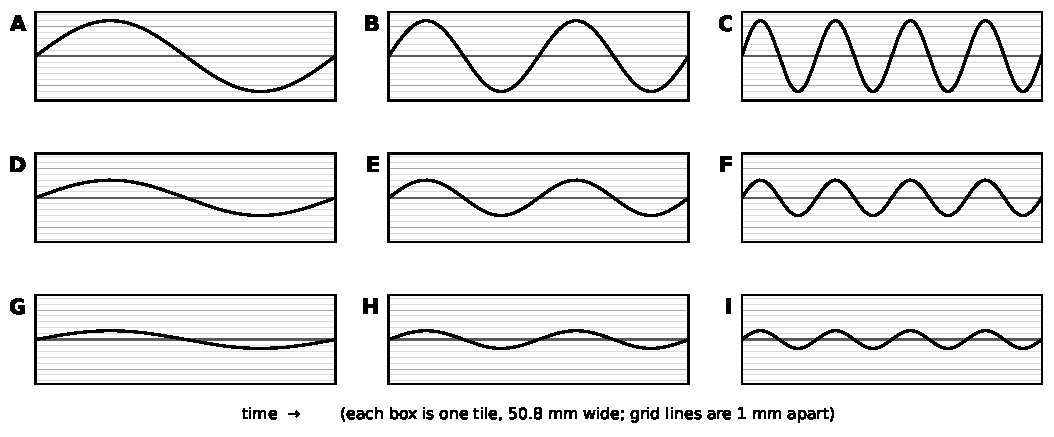
\includegraphics{profiles.pdf}
\end{center}

\noindent\textbf{Words to know.} A \textbf{cycle} is one complete up-and-down repeat of a wave. The
\textbf{amplitude} is how far a crest rises above the middle (zero) line. The \textbf{frequency}
is how many cycles happen each second; its unit is the \textbf{hertz} (Hz).

\begin{questions}

\question[9] For each tile, count the complete cycles and measure the amplitude in millimeters,
from the zero line to the top of a crest.

\begin{center}
\renewcommand{\arraystretch}{1.6}
\setlength{\tabcolsep}{7pt}
\begin{tabular}{|c|c|c||c|c|c||c|c|c|}
\hline
Tile & Cycles & Amp.\ (mm) & Tile & Cycles & Amp.\ (mm) & Tile & Cycles & Amp.\ (mm) \\ \hline
A & \ifprintanswers 1\fi & \ifprintanswers 6\fi & B & \ifprintanswers 2\fi & \ifprintanswers 6\fi & C & \ifprintanswers 4\fi & \ifprintanswers 6\fi \\ \hline
D & \ifprintanswers 1\fi & \ifprintanswers 3\fi & E & \ifprintanswers 2\fi & \ifprintanswers 3\fi & F & \ifprintanswers 4\fi & \ifprintanswers 3\fi \\ \hline
G & \ifprintanswers 1\fi & \ifprintanswers 1.5\fi & H & \ifprintanswers 2\fi & \ifprintanswers 1.5\fi & I & \ifprintanswers 4\fi & \ifprintanswers 1.5\fi \\ \hline
\end{tabular}
\end{center}
\begin{solution}
Measured values within about half a millimeter are fine. Each row shares one amplitude and each
column shares one cycle count.
\end{solution}

\question[2] Look across the top row, from A to C. What changes, and what stays the same?
\begin{solution}
The number of cycles increases (1, 2, 4), so the crests get closer together. The amplitude stays
the same (6~mm).
\end{solution}
\vspace{1.4cm}

\question[2] Look down the left column, from A to G. What changes, and what stays the same?
\begin{solution}
The amplitude gets smaller (6, 3, 1.5~mm). The number of cycles stays the same (1).
\end{solution}
\vspace{1.4cm}

\question[2] Which tile has the largest amplitude \emph{and} the most cycles? Which has the
smallest amplitude \emph{and} the fewest cycles?
\begin{solution}
C has both the largest amplitude and the most cycles. G has the smallest amplitude and the fewest
cycles.
\end{solution}
\vspace{1.0cm}

\question Suppose each tile shows exactly \textbf{one second} of a signal.
\begin{parts}
\part[3] What is the frequency of each column? Left: \blank[1.6cm]~Hz \quad Middle:
\blank[1.6cm]~Hz \quad Right: \blank[1.6cm]~Hz
\begin{solution}
1~Hz, 2~Hz, and 4~Hz.
\end{solution}
\part[2] The \textbf{period} is the time one cycle takes. What is the period of tile B? Of tile C?
\begin{solution}
B: 0.5~s (two cycles in one second). C: 0.25~s.
\end{solution}
\vspace{1.0cm}
\end{parts}

\question[3] In the box, sketch a tile with \textbf{3 cycles} and an \textbf{amplitude of 4~mm}.
Start at the zero line, going up, like the other tiles.
\begin{center}
\begin{tikzpicture}[x=1mm,y=1mm]
  \foreach \g in {-7,...,7} { \draw[gray!35, line width=0.2pt] (0,\g) -- (50.8,\g); }
  \draw[gray!80!black, line width=0.4pt] (0,0) -- (50.8,0);
  \draw[line width=0.5pt] (0,-7.5) rectangle (50.8,7.5);
  \ifprintanswers
    \draw[blue!60!black, line width=0.9pt, domain=0:50.8, samples=200] plot (\x, {4*sin(21.2598*\x)}); % 3 cycles in 50.8 mm = 1080/50.8 deg per mm
  \fi
\end{tikzpicture}
\end{center}

\question[2] A new tile has 8 cycles. Would its crests be closer together or farther apart than
tile C's? How far apart, in millimeters?
\begin{solution}
Closer together. The tile is 50.8~mm long, so 8 cycles put the crests \(50.8 / 8 \approx 6.4\)~mm
apart (tile C's are 12.7~mm apart).
\end{solution}
\vspace{1.4cm}

\question[2] If each tile were a sound, which tile would be the \textbf{loudest}? Which would have
the \textbf{highest pitch}? Explain.
\begin{solution}
Loudness goes with amplitude, so the top row (A, B, C) is loudest. Pitch goes with frequency, so
the right column (C, F, I) has the highest pitch. Tile C is both.
\end{solution}
\vspace{1.4cm}

\question[3] On the real board, a student runs a finger \emph{slowly} across tile C and
\emph{quickly} across tile A. The bumps can arrive at the fingertip at the same rate. Does that
mean A and C have the same frequency? Explain.
\begin{solution}
No. The frequency belongs to the signal: each tile stands for the same one second, and C fits
four cycles into it while A fits one. The finger's speed only changes how fast the student reads
the drawing, the way reading a graph quickly does not change the data. This is a limit of using
distance to stand for time.
\end{solution}
\vspace{2.0cm}

\question[2] Radio signals are waves too. Radio amateurs often talk on frequencies near 146~MHz
(megahertz). About how many cycles is that each second?
\begin{solution}
146~million cycles per second (\(1.46\times10^{8}\)).
\end{solution}
\vspace{1.0cm}

\newpage
\begin{center}
{\Large\bfseries Going further}\\[2pt]
{\normalsize For physics and engineering courses}
\end{center}

\question Let each tile now show \textbf{1~millisecond} (\SI{1}{ms}) of a signal.
\begin{parts}
\part[3] Find the frequency of each column, in hertz and kilohertz.
\begin{solution}
1000~Hz (1~kHz), 2000~Hz (2~kHz), and 4000~Hz (4~kHz).
\end{solution}
\vspace{1.0cm}
\part[2] Write the relationship between period \(T\) and frequency \(f\), and use it to find the
period of tile F.
\begin{solution}
\(T = 1/f\). Tile F has \(f = \SI{4}{kHz}\), so \(T = \SI{0.25}{ms}\).
\end{solution}
\vspace{1.4cm}
\end{parts}

\question The drawings could also show a wave \emph{in space} at one instant, with the horizontal
axis as distance. Then the spacing from crest to crest is the \textbf{wavelength} \(\lambda\), and
\(\lambda = v/f\), where \(v\) is the wave's speed.
\begin{parts}
\part[2] Sound in air at \SI{20}{\celsius} travels at about \SI{343}{m/s}. What is the wavelength
of a \SI{2}{kHz} tone?
\begin{solution}
\(\lambda = 343 / 2000 \approx \SI{0.17}{m}\) (17~cm).
\end{solution}
\vspace{1.4cm}
\part[2] Radio waves travel at the speed of light, about \SI{3.00e8}{m/s}. What is the wavelength
of a \SI{146}{MHz} signal? Why do radio amateurs call this the ``2-meter band''?
\begin{solution}
\(\lambda = 3.00\times10^{8} / 1.46\times10^{8} \approx \SI{2.05}{m}\). The band takes its name
from its wavelength, about 2~m.
\end{solution}
\vspace{1.6cm}
\part[2] Show that \(\lambda = vT\), and say in words what it means.
\begin{solution}
Since \(T = 1/f\), \(\lambda = v/f = vT\): in one period, the wave travels one wavelength.
\end{solution}
\vspace{1.4cm}
\end{parts}

\question[3] The power a wave carries is proportional to the square of its amplitude. How many
times more power does tile A carry than tile D? Than tile G?
\begin{solution}
A to D: \((6/3)^2 = 4\) times. A to G: \((6/1.5)^2 = 16\) times.
\end{solution}
\vspace{1.6cm}

\question[3] On the board, crest spacing (a distance) stands for the period (a time). Name one
thing a physical board cannot show about frequency, and propose a design change that would show
it.
\begin{solution}
Open-ended. A good answer notes that the board cannot make the signal itself change in time, so
the reader's hand sets the rate at which crests are felt. Possible changes include a moving part
(a rotating cam that lifts a pin at a fixed rate), a sound that plays with each tile, or a time
scale printed on the board.
\end{solution}
\vspace{2.2cm}

\end{questions}

\vfill
\noindent{\footnotesize Drafted with AI assistance (Claude) and reviewed by Nathaniel A. Frissell,
W2NAF. Source files, the 3D viewer, and print files:
\url{https://github.com/w3usr/handiham-tactile-aids}.}

\end{document}
